\documentclass[12pt,oneside,openany,a4paper, %... Layout
afrikaans,english,
%... Global lang drivers
]{memoir}
\usepackage[report, goldenblock]{usthesis}%... Thesis options
\usepackage[afrikaans, english]{babel}
%\SingleSpacing
\usepackage[left=3cm, right=2cm, top=2.5cm, bottom=2.5cm]{geometry}
\usepackage{amsmath}
\usepackage{mathtools}
\numberwithin{equation}{chapter}
\usepackage{bm}
\usepackage{graphicx}
\usepackage{subcaption}
\usepackage{color} % or xcolor
\usepackage{float} %figure location

\renewcommand{\thesection}{\thechapter.\arabic{section}}
\usepackage{tabto}

\usepackage{algorithm}
\usepackage{algpseudocode}
%Watermark
\usepackage{eso-pic}
\newcommand*{\WaterMark}[2][0.15\paperwidth]{%
\AddToShipoutPicture*{\AtTextCenter{%
\parbox[c]{0pt}{\makebox[0pt][c]{%
\includegraphics[width=#1]{#2}}}}}}

%References
\usepackage{usbib}%............................. Bibliography
\bibliographystyle{usmeg-n}%................. Auhor-year style
\addto{\captionsenglish}{\renewcommand{\bibname}{List of References}}

\begin{document}
\pagestyle{plain}
\frontmatter
%TiltePage:
\title{Numerical integration for probabilisitc reasoning skripsie}
\author{JM.\ Louw}{Jacobus Martin Louw}
\faculty{Faculty of Electrical and Electronic Engineering}
\degree{BEng (E&E)}{Bachelor of Engineering (Electrical and Electronic)}
\ReportDescript{Final Report}
\supervisor{Dr\ CE\ van Daalen}
\frontmatter
\WaterMark{UScrest-WM}
\TitlePage

\addtocontents{toc}{\protect\setcounter{tocdepth}{-1}}
%Declaration Page
\DeclarationPage

%abstract
\address{Department of Electrical and Electronic Engineering,\\
University of Stellenbosch,\\
Private Bag X1, 7602 Matieland, South Africa.}
\newpage

\tableofcontents
\addtocontents{toc}{\protect\setcounter{tocdepth}{2}}
\pagebreak
\listoffigures

\chapter{List of Acronyms}

\begin{tabbing}
\hspace*{1em}\= \hspace*{5em} \= \hspace*{3em} \= \kill % set the tabbings
\> CPD	\> - \> conditional probability distribution\\
\> EKF	\> - \> extended Kalman filter\\
\> KF	\> - \> Kalman filter\\
\> PDF	\> - \> probability density function\\
\> PGM	\> - \> probabilistic graphical model\\
\> RV \> - \>	random variable\\
\> UKF	\> - \> unscented Kalman filter\\
\end{tabbing}

\chapter{List of Notations}
\begin{tabbing}
\hspace*{1em}\= \hspace*{5em} \= \hspace*{3em} \= \kill % set the tabbings
\> $x$	\> - \> scalar\\
\> $\bm{x}$	\> - \> vector\\
\> $\bm{x}^T$	\> - \> transpose of vector\\
\> $X$ \> - \> matrix\\
\> $X^T$ \> - \> transpose of matrix\\
\> $X^{-1}$ \> - \> inverse of matrix\\
\> $|X|$ \> - \> determinant of matrix\\
\> $p(x)$ \> - \> probability density function\\
\> $\mathcal{N}(\bm{x}; \bm{\mu}, \Sigma)$ \> - \> covariance form\\
\> $\mathcal{C}(\bm{x}; K, \bm{h})$ \> - \> canonical form
\end{tabbing}

\chapter{List of Symbols}
\begin{tabbing}
\hspace*{1em}\= \hspace*{5em} \= \hspace*{3em} \= \kill % set the tabbings
\> $C$	\> - \> cluster\\
\> $\bm{h}$	\> - \> potential vector\\
\> $K$	\> - \> information matrix\\
\> $\delta$ \> - \> message in a cluster graph\\
\> $\eta$ \> - \> normalisation coefficient\\
\> $\psi$ \> - \> initial belief cluster\\
\> $\Sigma$ \> - \> covariance matrix
\end{tabbing}
\begin{abstract}
Text in default language ...
\end{abstract}


\mainmatter
\chapter{Introduction}
Robot localisation is the process of estimating where a robot is located relative to its environment. It is essential for autonomous robots to have precise knowledge of their location in order to navigate their surroundings.

When localising a robot, the control input to the robot, and a map of the environment is usually available. Further the robot is generally fitted with sensors which, together with beacons, measure where the robot is located relative to the map. Unfortunately the information of the robot's movements and location always have noise to some degree.\\
The position and orientation of the robot should rather be estimated in a probabilistic manner from the information gathered from the sensors. The localisation techniques must therefore be able to deal with noise and describe the robot's location with a measure of uncertainty.\\
Probabilistic reasoning of systems with continuous random variables (RV) use integration for various operations. In most non-linear systems these integrals cannot be calculated analytically and one must use numerical methods. Kalman filters have been extensively used for localisation. Techniques such as the extended or unscented Kalman filters use primitive numerical integration that is very inaccurate, especially when measurements are also non-linear. However, there are several alternative numerical techniques available that are more accurate.

A probabilistic graphical model (PGM) is a technique that is used to model systems with uncertainty in an organised manner. It describes the relationship between random variables and allows to reason about their likelihood based on knowledge that is available to the system. Reasoning about random variables in a PGM consists of a number of steps and one can easily identify where integration is used.

The end goal of this project is investigate different numerical techniques of integration and to implement them in a PGM to localise a simulated robot. The accuracy and efficiency of different techniques of numerical integration when used to inference a non-linear system will be compared using a simulated environment.
\setcounter{secnumdepth}{2}
\chapter{Gaussian Random Variables}
The Gaussian or normal distribution is commonly used in probability theory, as it is very easy to work with. Although Gaussian distributions make severe assumptions such as exponential decay of the distribution away from its mean and linear interactions between variables, they are often surprisingly good estimations for real world distributions. The Gaussian distribution is a very important concept in this report as all probability distributions are approximated as Gaussian distributions. Key concepts, features and representations of the Gaussian distribution are discussed in this chapter. The following chapter is based on the work of Peebles and Shi~\cite{peebles} and Koller and Friedman~\cite{koller}.

\section{Covariance form}
Random variables can take different values described by some function. A Gaussian RV is a RV which value is drawn from Gaussian distribution.

The univariate Gaussian distribution is probability density function (PDF) of a single Gaussian RV. The covariance form fully describes a univariate Gaussian distribution by a mean $\mu$ and variance $\sigma^2$.
The univariate Gaussian distribution of a RV $x$, denoted
\begin{equation}
x\sim\mathcal{N}(\mu,\sigma),
\end{equation}
has a PDF that is defined by
\begin{equation}\label{eq:1}
p(x) = \eta\exp\left[\frac{-(x-\mu)^2}{2\sigma^2}\right],
\end{equation}
with a normalisation coefficient 
\begin{equation}\label{eq:2}
\eta = \frac{1}{\sqrt{2\pi\sigma^2}}.
\end{equation}
The mean parameter $\mu$ describes the location of the peak of the distribution and the variance parameter $\sigma^2$ describes the tempo which the distribution decays. The probability to draw of a value $X$ out of a Gaussian distribution decreases exponentially as the value of $X$ moves farther from the mean. The standard deviation of the Gaussian distribution is denoted as $\sigma$ and is an indication of the spread of the graph.

If $x$ is a continuous RV, then the mean or expectation of $x$ is
\begin{equation}
\mu = E\left[ x \right] = \int x \cdot p(x)dx.
\end{equation}
The variance of $x$ can be calculated as
\begin{equation}
\begin{split}
\sigma^2 & = E\left[\left(x - E[x]\right)^2\right]\\
& = E[x^2] - (E[x])^2
\end{split}
\end{equation}
 Figure \ref{fig:gPDF1} indicates the mean $\mu$ and standard deviation $\sigma$ of an univariate Gaussian PDF.
\begin{figure}[H]
  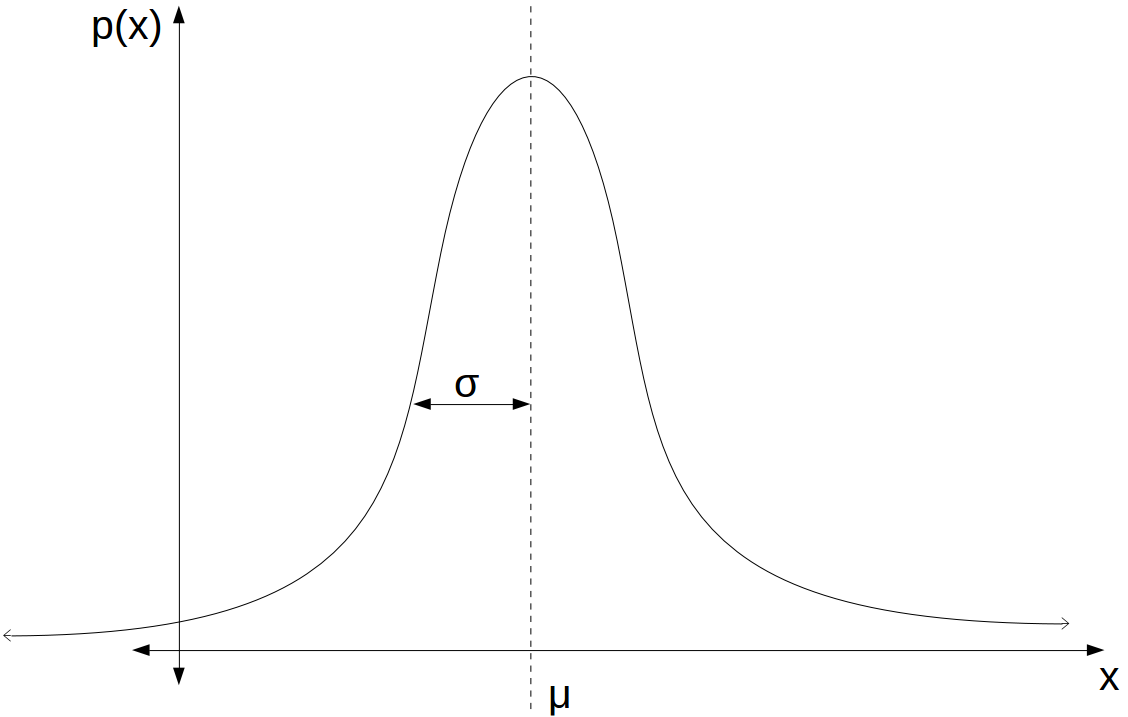
\includegraphics[width=0.6\linewidth]{Figures/univariate.png}
  \centering
  \caption{Univariate Gaussian PDF}
  \label{fig:gPDF1}
\end{figure}
The definition of the Gaussian distribution can be extended to describe the PDF of $N$ random variables, this is called the multivariate Gaussian distribution. The multivariate Gaussian distribution is described by an $N$-dimensional mean vector $\bm{\mu}$ and an $N\times N$ covariance matrix $\Sigma$. The multivariate Gaussian distribution of a set of $N$ random variables,  or random vector
\begin{equation}
\bm{x} = [x_1\ ...\ x_N]^T,
\end{equation}
is denoted as
\begin{equation}
\bm{x} \sim \mathcal{N}(\bm{x}; \bm{\mu},\Sigma),
\end{equation}
and it has a PDF that is described by
\begin{equation}\label{eq:3}
p(\bm{x})  = \eta\exp\left[-\frac{1}{2}(\bm{x}-\bm{\mu})^T\Sigma^{-1}(\bm{x}-\bm{\mu})\right],
\end{equation}
with a normalisation coefficient
\begin{equation}\label{eq:4}
\eta = \frac{1}{(2\pi)^{\frac{N}{2}}|\Sigma|^{\frac{1}{2}}}.
\end{equation}
$|\Sigma|$ is the the determinant of $\Sigma$.

For this report it is required that $\Sigma$ is positive definite and thus also non-singular, which guarantees a determinant that is non-zero. Positive definite covariance matrices are also invertible, thus the alternative canonical or information form, which requires $\Sigma^{-1}$, can be used. The canonical form is discussed in the following section.

The mean vector of RV vector $\bm{x}$ is equal to the expectation of $\bm{x}$ and is defined as
\begin{equation}
\bm{\mu} = E[\bm{x}].
\end{equation}
The covariance matrix $\Sigma$ specifies the correlation between RVs and is equal to
\begin{equation}
\Sigma = E[\bm{xx}^T] - E[\bm{x}]E[\bm{x}]^T.
\end{equation}
\subsection{Error ellipse}The following section is based on an article by Abdi ~\cite{abdi} and on a webpage from "Computer vision for dummies"~\cite{draw_ellipse}.

A multivariate Gaussian distribution with RV vector
\begin{equation}
\bm{x} = [x_1\ x_2]^T
\end{equation}
can be visualised as a series of ellipsoidal contours around the mean vector $\bm{\mu}$. The contours are an indication of the correlation between $x_1$ and $x_2$ and also show the uncertainty of the PDF. Contours close to each other suggest a steep incline and contours farther apart suggest a gradual incline in the PDF. Hence, small and concentrated contours represent confident Gaussian distributions and contours that are larger and further apart represent uncertain Gaussian distributions. Error ellipsis are an effective way to indicate the mean, uncertainty and correlation of 2D Gaussian distributions.

An ellipse has a major axis and a minor axis as shown in Figure \ref{fig:e_ellipse}. The major axis of the error ellipse is always aligned in the direction the Gaussian distribution varies most. This direction can be found by determining the eigenvectors of the distribution. Each eigenvector has a corresponding eigenvalue which indicates the spread of the distribution in the direction of the eigenvector. 

We can use eigenvalue decomposition to factorise the covariance matrix $\Sigma$,
\begin{equation}
\Sigma = Q\Lambda Q^{-1}.
\end{equation}
Each column of the eigenvector matrix $Q$ contains an eigenvector $\bm{v}$. $Q$ is defined as
\begin{equation}
Q =
[\bm{v_1} \ \bm{v_2}]
=
\begin{bmatrix}
v_{11} & v_{21}\\
v_{12} & v_{22}
\end{bmatrix}.
\end{equation}
$\Lambda$ is a diagonal matrix and each of its diagonal entries contains an eigenvalue $\lambda$. $\Lambda$ is defined as 
\begin{equation}
\Lambda =
\begin{bmatrix}
\lambda_1 & 0\\
0 & \lambda_2
\end{bmatrix}.
\end{equation}
An error ellipsis of a Gaussian PDF can be specified in terms of confidence levels which is the probability that a value drawn from the distribution will fall inside the ellipse. Thus, differently sized ellipsis can be plotted for different confidence levels. The lengths of the major an minor axes are sequentially specified as $2\sqrt{s\lambda_1}$ and $2\sqrt{s\lambda_2}$, where $\lambda_1 \geq \lambda_2$. The value of $s$ is determined by the confidence level of the error ellipse. In the case of an error ellipse with a confidence level of 95\%, $s$ is set to 5.991. The Chi-Square distribution can be used to find $s$ for other confidence levels, but it is beyond the scope of this document.

The orientation $\alpha$ of the error ellipse is shown in Figure \ref{fig:e_ellipse}. To obtain $\alpha$ we calculate the angle, relative to the x-axis, of the eigenvector with the largest spread. The angle $\alpha$ is defined as
\begin{equation}
\alpha = \arctan\left(\frac{v_{11}}{v_{12}}\right),
\end{equation}
where $\lambda_1 \geq \lambda_2$.

\begin{figure}[H]
  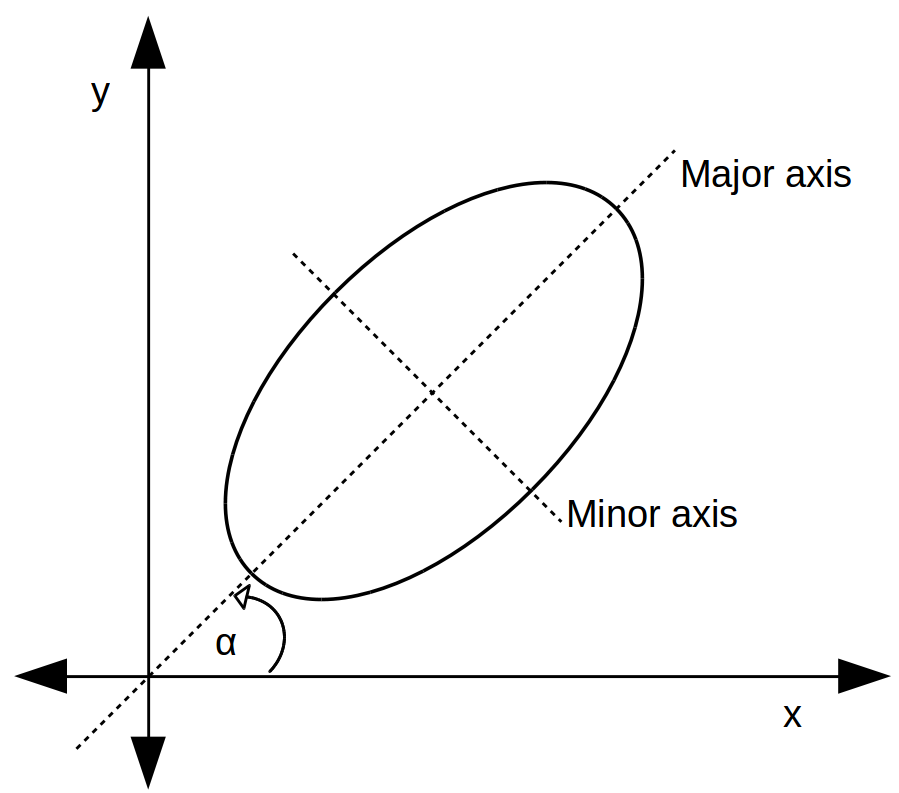
\includegraphics[width=0.5\linewidth]{Figures/e_ellipse.png}
  \centering
  \caption{Error Ellipse}
  \label{fig:e_ellipse}
\end{figure}
\section{Canonical form}
The canonical or information form is an alternative way to describe Gaussian distributions. Using the canonical form has benefits, such as certain operations are easier to perform. It can also be used to represent Gaussian conditional probability densities (CPDs), which will be discussed later in this section. The following section is based on the work of Koller and Friedman~\cite{koller} and Schoeman~\citep{JC}.

Equation \ref{eq:3}, which is the definition of a Gaussian PDF, can be rewritten
\begin{equation}
\begin{split}\label{eq:6}
p(\bm{x}) & = \eta\exp\left[-\frac{1}{2}(\bm{x}-\bm{\mu})^T\Sigma^{-1}(\bm{x}-\bm{\mu})\right]\\
& = \exp\left(-\frac{1}{2}\bm{x}^T\Sigma^{-1}\bm{x} + \bm{\mu}^T\Sigma^{-1}\bm{x} - \frac{1}{2}\bm{\mu}^T\Sigma^{-1}\bm{\mu} + \ln{\eta}\right),
\end{split}
\end{equation}
with the information matrix
\begin{equation}\label{eq:7}
K = \Sigma^{-1},
\end{equation}
the potential vector
\begin{equation}\label{eq:8}
\bm{h} = \Sigma^{-1}\bm{\mu},
\end{equation}
and scalar
\begin{equation}\label{eq:9}
g = - \frac{1}{2}\bm{\mu}^T\Sigma^{-1}\bm{\mu} + \ln{\eta}.
\end{equation}
Thus the definition of the canonical form is
\begin{equation}\label{eq:canonical}
\mathcal{C}(\bm{x}; K,\bm{h},g) = \exp\left(-\frac{1}{2}\bm{x}^TK\bm{x} + \bm{h}^T\bm{x} +g \right).
\end{equation}
As one can always determine $g$ from $\bm{h}$ and $K$, the canonical form can be described as
\begin{equation}
\mathcal{C}(\bm{x}; K,\bm{h},g) \propto \mathcal{C}(\bm{x}; K,\bm{h}).
\end{equation}
The covariance parameters can easily be recovered:
\begin{equation}
\Sigma = K^{-1}
\end{equation}
\begin{equation}
\bm{\mu} = \Sigma\bm{h}
\end{equation}
IF $K$ is not invertible and the covariance can not be recovered, the canonical form is therefore more general than the covariance form.

It can be seen from the above that it is very easy to convert between the canonical an covariance form. 
\subsection{Operations using the Canonical Form}
This section will cover useful operations using the canonical form. 

Extending and rearranging scopes of canonical forms may be necessary before doing operations, as it is important that scopes of canonical forms are identical when doing operations. 
\subsubsection{Extending the Scope of a Canonical Form:}
The scope of a canonical form can be extended by adding zero entries to $K$ and $\bm{h}$:
\begin{equation}
\mathcal{C}\left(
\begin{bmatrix}
\bm{x}\\
\bm{y}
\end{bmatrix};
\begin{bmatrix}
K_{\bm{xx}} & K_{\bm{xy}}\\
K_{\bm{yx}} & K_{\bm{yy}}
\end{bmatrix},
\begin{bmatrix}
\bm{h_x}\\
\bm{h_y}
\end{bmatrix}
\right)
=
\mathcal{C}\left(
\begin{bmatrix}
\bm{x}\\
\bm{y}\\
\bm{z}
\end{bmatrix};
\begin{bmatrix}
K_{\bm{xx}} & K_{\bm{xy}} & \textit{0}\\
K_{\bm{yx}} & K_{\bm{yy}} & \textit{0}\\
\textit{0} & \textit{0} & \textit{0}
\end{bmatrix},
\begin{bmatrix}
\bm{h_x}\\
\bm{h_y}\\
\textit{0}
\end{bmatrix}
\right)
\end{equation}
\subsubsection{Rearranging the Scope of a Canonical Form:}
The scope can be rearranged by rearranging the rows and columns of $K$  and rearranging the entries of $\bm{h}$:
\begin{equation}
\mathcal{C}\left(
\begin{bmatrix}
\bm{x}\\
\bm{y}\\
\bm{z}
\end{bmatrix};
\begin{bmatrix}
K_{\bm{xx}} & K_{\bm{xy}} & K_{\bm{xz}}\\
K_{\bm{yx}} & K_{\bm{yy}} & K_{\bm{yz}}\\
K_{\bm{zx}} & K_{\bm{zy}} & K_{\bm{zz}}
\end{bmatrix},
\begin{bmatrix}
\bm{h_x}\\
\bm{h_y}\\
\bm{h_z}
\end{bmatrix}
\right)
=
\mathcal{C}\left(
\begin{bmatrix}
\bm{y}\\
\bm{x}\\
\bm{z}
\end{bmatrix};
\begin{bmatrix}
K_{\bm{yy}} & K_{\bm{yx}} & K_{\bm{yz}}\\
K_{\bm{xy}} & K_{\bm{xx}} & K_{\bm{xz}}\\
K_{\bm{zy}} & K_{\bm{zx}} & K_{\bm{zz}}
\end{bmatrix},
\begin{bmatrix}
\bm{h_y}\\
\bm{h_x}\\
\bm{h_z}
\end{bmatrix}
\right)
\end{equation}
\subsubsection{Multiplication of Canonical Forms:}
If the scopes of two canonical forms are identical, one can multiply them by simply summing the $K$ and $\bm{h}$ parameters of the two canonical forms:
\begin{equation}\label{eq:10}
\mathcal{C} (\bm{x}; K_{\bm{x}},\bm{h_x}) \times \mathcal{C} (\bm{y}; K_{\bm{y}},\bm{h_y})= \mathcal{C} (\bm{z};K_{\bm{x}} + K_{\bm{y}}, \bm{h_x} + \bm{h_y})
\end{equation}
%\subsubsection{Division of canonical forms:}
%Again, it important that the scopes of the distributions are identical.
%\begin{equation}\label{eq:11}
%\frac{\mathcal{C}(K_1,\bm{h_1},g_1)}{\mathcal{C}(K_2,\bm{h_2},g_2)} = %\mathcal{C}(K_1 - K_2,\bm{h_1} - \bm{h_2},g_1 - g_2)
%\end{equation}
\subsubsection{Marginalisation of a Canonical Form:}
A marginal distribution can be found by integrating over a subset of variables. For example the marginal distribution over $\bm{x}$ can be found by integrating over $\bm{y}$. Let $\mathcal{C}(\bm{x},\bm{y};K,\bm{h},g)$ be a canonical form with subsets $\bm{x}$ and $\bm{y}$ where
\begin{equation}
K = 
\begin{bmatrix}
K_{\bm{xx}} & K_{\bm{xy}}\\
K_{\bm{yx}} & K_{\bm{yy}}
\end{bmatrix}
\end{equation}
and
\begin{equation}
\ h = 
\begin{pmatrix}
h_{\bm{x}} \\
h_{\bm{y}}
\end{pmatrix}.
\end{equation}
To obtain the marginal distribution over $\bm{x}$, we have to find the integral over $\bm{y}$. Therefore the marginal distribution over $\bm{x}$ is
\begin{equation}
\int\mathcal{C}(\bm{x},\bm{y};K,\bm{h},g)d\bm{y} = \mathcal{C}(\bm{x};K',\bm{h}',g'),
\end{equation}
 where
\begin{equation}
K' = K_{\bm{xx}} - K_{\bm{xy}}K_{\bm{yy}}^{-1}K_{\bm{yx}},
\end{equation}
\begin{equation}
\bm{h'} = \bm{h}_{\bm{x}} - K_{\bm{xx}}K_{\bm{yy}}^{-1}\bm{h}_{\bm{y}}
\end{equation}
and
\begin{equation}
g' = g - \frac{1}{2}\left(\ln|2\pi K_{\bm{yy}}^{-1}|+ \bm{h_y}^T K_{\bm{yy}}^{-1}\bm{h_y}\right).
\end{equation}
It is important to that $K_{\bm{yy}}$ is positive-definite for the result to be finite.
\subsubsection{Reduction with Evidence:}
Let $\mathcal{C}(\bm{x},\bm{y};K,\bm{h},g)$ be a canonical form with subsets $\bm{x}$ and $\bm{y}$. If the value of subset $\bm{y}$ is known to be $\bm{Y}$, then the canonical form can be reduced to $\mathcal{C}(\bm{x}; K',\bm{h}',g')$, where
\begin{equation}
K' = K_{\bm{xx}},
\end{equation}
\begin{equation}
\bm{h'} = \bm{h}_{\bm{x}} - K_{\bm{xy}}\bm{Y},
\end{equation}
and
\begin{equation}
g' = g + \bm{h}_{\bm{y}}^T\bm{Y} - \frac{1}{2}\bm{Y}^TK_{\bm{yy}}\bm{Y}.
\end{equation}
The operations discussed above are very simple to perform and will be used in following chapters.
\subsection{Linear Transformations using the Canoncical Form}
One of the advantages of the canonical form is that it is possible to represent conditional probability distributions.

The CPD $p(\bm{y}|\bm{x})$ is the distribution of the vector $\bm{y}$ given we know that the distribution over the vector $\bm{x}$ and is defined as
\begin{equation}
p(\bm{y}|\bm{x}) = \frac{p(\bm{y},\bm{x})}{p(\bm{y})}.
\end{equation}

If a CPD such as $p(\bm{y}|\bm{x})$ can be described as a linear transform
\begin{equation}
\bm{y} = F\bm{x} + \bm{g} + \bm{n},
\end{equation}
where
\begin{equation}
\bm{n} \sim \mathcal{N}(\bm{n}; \bm{0}, \Sigma_n).
\end{equation}
The probability distribution is
\begin{equation}
\label{eq:30}
\begin{split}
p(\bm{y}|\bm{x}) & = \mathcal{N}(\bm{y}; F\bm{x} + \bm{g}, \Sigma) \\
& = \eta\exp\left[-\frac{1}{2}(\bm{y} - (F\bm{x} + \bm{g}))^T\Sigma^{-1}(\bm{y}-(F\bm{x} + \bm{g}))\right].
\end{split}
\end{equation}
A part of Equation \ref{eq:30} can be rewritten as 
\begin{equation}\label{eq: rewrite}
\begin{split}
\bm{y} - (F\bm{x} + \bm{g}) & =
\begin{bmatrix}
I&-F&-I
\end{bmatrix}
\begin{bmatrix}
\bm{y}\\
\bm{x}\\
\bm{g}
\end{bmatrix}\\
& =
\begin{bmatrix}
I\\-F^T\\-I
\end{bmatrix}^T
\begin{bmatrix}
\bm{y}\\
\bm{x}\\
\bm{g}
\end{bmatrix}.
\end{split}
\end{equation}
Substituting Equation \ref{eq: rewrite} into Equation \ref{eq:30} gives
\begin{equation}
\label{eq:32}
\begin{split}
p(\bm{y}|\bm{x}) = \eta\exp\left[-\frac{1}{2}
\begin{bmatrix}
\bm{y}\\
\bm{x}\\
\bm{g}
\end{bmatrix}^T
\begin{bmatrix}
I\\-F^T\\-I
\end{bmatrix}
\Sigma^{-1}
\begin{bmatrix}
I\\-F^T\\-I
\end{bmatrix}^T
\begin{bmatrix}
\bm{y}\\
\bm{x}\\
\bm{g}
\end{bmatrix}
\right].
\end{split}
\end{equation}
Defining a combined random vector
\begin{equation}\label{eq:ranVec}
\bm{w} = 
\begin{bmatrix}
\bm{y}\\
\bm{x}\\
\bm{g}

\end{bmatrix}
\end{equation}
and information matrix
\begin{equation}\label{eq:newK}
K' =
\begin{bmatrix}
I\\-F^T\\-I
\end{bmatrix}
\Sigma^{-1}
\begin{bmatrix}
I\\-F^T\\-I
\end{bmatrix}^T.
\end{equation}
We can substitute Equation \ref{eq:ranVec} and Equation \ref{eq:newK} into Equation \ref{eq:32} which gives
\begin{equation}
\label{eq:35}
\begin{split}
p(\bm{y}|\bm{x}) = \eta\exp\left[-\frac{1}{2}
\bm{w}^T
K'
\bm{w}
\right].
\end{split}
\end{equation}
We can now use Equation \ref{eq:canonical} to write the conditional distribution of Equation \ref{eq:35} in the canonical form as follows
\begin{equation}
\begin{split}
p(\bm{y}|\bm{x}) & \propto \mathcal{C}(\bm{w}: K', \bm{0})\\
& =\mathcal{C}\left(
\begin{bmatrix}
\bm{y} \\
\bm{x} \\
\bm{g}
\end{bmatrix};
\begin{bmatrix}
I\\
-F^T\\
-I
\end{bmatrix}
\Sigma_n^{-1}
\begin{bmatrix}
I & -F & -I
\end{bmatrix}, \bm{0}, -
\right)\\
& =\mathcal{C}\left(
\begin{bmatrix}
\bm{y} \\
\bm{x} \\
\end{bmatrix};
\begin{bmatrix}
I\\
-F^T
\end{bmatrix}
\Sigma_n^{-1}
\begin{bmatrix}
I & -F
\end{bmatrix},
\begin{bmatrix}
I\\
-F^T
\end{bmatrix}
\Sigma_n^{-1}\bm{g}, -
\right)\\
& =\mathcal{C}\left(
\begin{bmatrix}
\bm{y} \\
\bm{x} \\
\end{bmatrix};
\begin{bmatrix}
\Sigma_n^{-1}  &  -\Sigma_n^{-1}F\\
-F^T\Sigma_n^{-1} & F^T\Sigma_n^{-1}F
\end{bmatrix}
, 
\begin{bmatrix}
-\Sigma_n^{-1}\bm{g}\\
-F^T\Sigma_n^{-1}\bm{g}
\end{bmatrix},
-
\right).
\end{split}
\end{equation}
This representation of conditional probability densities in the canonical form will be very useful in future chapters.
\chapter{Motion models}
Before implementing a localisation algorithm to localise a robot, it is important to have a model which describes the movement of the robot. A simple linear motion model will be covered which will later be used to illustrate basic principles when localising linear moving objects. A more complex non-linear motion model will be explored which will be essential when investigating numerical integration techniques for localising non-linear moving objects. This chapter is based on the work of S. Thrun, W. Burgard and D. Fox~\citep{thrun};
\section{Basic concepts}
The motion model describes $p(x_t|u_t,x_{t-1})$, which is the transition probability and it is vital in the the prediction step of the Bayes filter. The material will cover kinematics in a stochastic form. Robot motion will be limited to planar movement as it is easier to convey concepts or ideas to the reader. Note that the theory discussed is not limited to planar movement.

The kinematic state of a robot moving in a plane can be described by three variables which is referred to as the pose of the robot.
The pose is defined as
\begin{equation}
\bm{x_t} =
\begin{bmatrix}
x_t\\
y_t\\
\theta_t
\end{bmatrix},
\end{equation}
where $x_t$ is the x-coordinate, $y_t$ is the y-coordinate and $\theta_t$ is the orientation of the robot at time $t$. 
\section{Linear Motion Model}
The linear motion model describes linear movement of a robot between time steps in a plane. The parameter $\theta_t$ is omitted from the pose  and therefore the kinematic state of the robot is described by only a location
\begin{equation}
\bm{x_t} =
\begin{bmatrix}
x_t\\
y_t
\end{bmatrix},
\end{equation}
which allows the model to be linear.

The linear motion model used in this project describes the movement of the robot with a control vector which contains two translational velocities
\begin{equation}
\bm{u_t} = 
\begin{bmatrix}
v_{x,t}\\
v_{y,t}
\end{bmatrix},
\end{equation}
where $v_{x,t}$ is the velocity in the x-direction and $v_{y,t}$ is the velocity in the y-direction at time $t$.

The position of the robot at time $t$ can be described as linear function in the form of
\begin{equation}
\bm{x_t} = A \bm{x_{t - 1}} + B \bm{u_t} + \bm{n},
\end{equation}
where
\begin{equation}
A =
\begin{bmatrix}
1 & 0\\
0 & 1
\end{bmatrix},
\end{equation}
\begin{equation}
B = \begin{bmatrix}
\Delta t & 0\\
0 & \Delta t
\end{bmatrix},
\end{equation}
\begin{equation}
\bm{n} =
\begin{bmatrix}
n_x\\
n_y
\end{bmatrix},
\end{equation}
and the noise is described as Gaussian distributions
\begin{equation}
n_x \sim \mathcal{N}(n_x; 0, \sigma_x^2),
\end{equation}
\begin{equation}
n_y \sim \mathcal{N}(n_y; 0, \sigma_y^2).
\end{equation}
The variances $\sigma_x^2$ and $\sigma_y^2$ is determined empirically and $\Delta t$ is the length of a time step.


\section{Non-linear Motion Model}
Two non-linear motion models were considered for this project, namely the velocity and odometry model. The odometry motion model uses sensor measurements to describe a robot's motion over time as a rotation, translation and then another rotation. Odometry models can only be used for retrospect after a robot moved and can not be used for motion planning. The velocity model is suitable for motion planning and assumes that a robot can be controlled with a rotational and translational velocity. The odometry model is usually more accurate than the velocity model, as it is difficult to get an accurate reading of the revolution of a robot's wheels. The velocity motion model was used in this project as it more relevant to motion planning for autonomous robots.

The velocity motion model assumes that the movement of a robot can be described by a translational velocity $v_t$ and a rotational velocity $\omega_t$ . The control vector $u_t$ is thus described as
\begin{equation}
\bm{u_t} = 
\begin{bmatrix}
v_t\\
\omega_t
\end{bmatrix}.
\end{equation}
Positive rotational velocities are defined to be counter-clockwise and positive translational velocities are specified to be in the "forward" direction.
The position $x_t$ and $y_t$, and orientation $\theta_t$ at time $t$ can be determined
\begin{equation}
x_t = x_{t-1} - \frac{v_t}{\omega_t} \sin\theta_{t-1} + \frac{v_t}{\omega_t} \sin(\theta_{t-1} + \omega_t \Delta t) + n_x
\end{equation}
\begin{equation}
y_t = y_{t-1} - \frac{v_t}{\omega_t} \cos\theta_{t-1} + \frac{v_t}{\omega_t} \cos(\theta_{t-1} + \omega_t \Delta t) + n_y
\end{equation}
\begin{equation}
\theta_t = \theta_{t-1} + \omega_t \Delta t + n_\theta,
\end{equation}
where
\begin{equation}
n_x \sim \mathcal{N}(n_x; 0, {\sigma_x}^2),
\end{equation}
\begin{equation}
n_y \sim \mathcal{N}(n_y; 0, {\sigma_y}^2)
\end{equation}
and
\begin{equation}
n_\theta \sim \mathcal{N}(n_\theta; 0, {\sigma_\theta}^2).
\end{equation}
Where variances ${\sigma_x}^2$, ${\sigma_x}^2$ and ${\sigma_x}^2$ are determined empirically.

The model is non-linear due to the fact due to the fact that the movement of the robot cannot be described by a linear translation in the form of
\begin{equation}
\bm{y} = A\bm{x} + B
\end{equation}
\chapter{Measurement Models}

As mentioned in the introduction, measurements retrieved from sensors always contain noise. A measurement model can be used one can describe it with a model. This chapter will describe the linear measurement model and is based on Thrun~\citep{thrun}.
\section{Linear Measurement Model}

\chapter{Localisation using Kalman Filters}
This chapter will focus on localisation using traditional techniques such as the Kalman filter, extended Kalman filter and unscented Kalman filter. This is important to investigate and understand as there is a strong correspondence to the PGM technique that will be discussed in a following section
\section{Background}
A concept that is often used is in this report is that of \textit{belief}. As mentioned in the introduction, a robot cannot truly know its pose. A robot can infer a belief or have internal knowledge of its state from information gathered from sensors. There is thus a difference between internal belief and true state.

Beliefs are represented with CPDs. A belief is thus a PDF of a state variable which is conditioned on given data. The belief of a state variable is denoted as
\begin{equation}
x_t \sim bel(x_t)
\end{equation}
which a reduced notation for the posterior
\begin{equation}
bel(x_t) = p(x_t| z_{1:t}, u_{1:t})
\end{equation}
The posterior is the PDF of a state variable $x_t$ at time $t$ conditioned on all the previous control inputs $u_{1:t}$ and measurements $z_{1:t}$. The posterior $bel(x_t)$ is usually calculated from a \textit{predicted belief} $\overline{bel}(x_t)$, this calculation is known as the \textit{update step}.

The \textit{predicted belief} is defined as
\begin{equation}
\overline{bel}(x_t) = p(x_t|z_{1:t-1}, u_{1:t}),
\end{equation} 
and is the PDF of the state variable $x_t$ without taking the measurement $z_t$ in to consideration, hence it is known as the \textit{prediction step}.
\section{Bayes Filter}
The \textit{Bayes Filter} algorithm is the cornerstone for determining beliefs and filters such as the Kalman filter is a variation of it. The pseudo code for the Bayes filter is shown in Algorithm \ref{bayesAlg}. One can observe that the algorithm is recursive as it takes the previous belief $x_{t-1}$ at time $t-1$ as an argument to estimate and return the belief $x_t$ at time $t$. The algorithm takes three parameters, namely the previous belief $bel(x_{t-1})$, the latest control input $u_t$ and, the measurements $z_t$ which is a result of the control input. The pseudo code shows one iteration of the algorithm which consist out of two steps, namely the \textit{prediction step} in line 3, and \textit{update step} in line 4.

The \textit{prediction step} calculates a belief of the state $x_t$ based on the previous state $x_{t-1}$ and the control input $u_t$. In this step the marginal distribution over $x_{t-1}$ is calculated of the product of two distributions: the prior belief $bel(x_{t-1})$, and the PDF of $x_t$ given $u_t$ and $x_{t-1}$.

In the \textit{update step} the final belief of state $x_t$ is calculated by multiplying the predicted belief $\overline{bel}(x_t)$ with the probability of $z_t$ given $x_t$. The result usually does not integrate to one, hence it is not a valid PDF and has to be normalized with $\eta$. The final belief $bel(x_t)$ is returned.
\begin{algorithm}
\caption{Bayes Filter}\label{bayesAlg}
\begin{algorithmic}[1]
\Procedure{Bayes\_Filter}{$bel(x_{t-1}), u_t, z_t$}
\ForAll{$x_t$}
\State $\overline{bel}(x_t) = \int p(x_t|u_t, x_{t-1})bel(x_{t-1})\, dx_{t-1}$
\State $bel(x_t) = \eta p(z_t|x_t) \overline{bel} (x_t)$
\EndFor
\State \textbf{return} $bel(x_t)$
\EndProcedure
\end{algorithmic}
\end{algorithm}

\section{Kalman Filter}
The Kalman filter is an implementation of the Bayes filter and is used for prediction in linear Gaussian systems. The Kalman filter is used in systems data is continuously changing and it is not applicable in discrete state spaces. The Kalman filter makes three assumptions in addition to the Markov assumptions which have the outcome that posterior beliefs calculated with the Kalman filter are Gaussian distributions.

1.Linear system dynamics are assumed. The motion model describing the movement must be linear with added Gaussian noise $\bm{n}$ and must be able to express it with 
\begin{equation}
\bm{x}_t = A \bm{x}_{t - 1} + B \bm{u}_t + \bm{\varepsilon},
\end{equation}
with 
\begin{equation}
\bm{\varepsilon} \sim \mathcal{N}(\bm{\varepsilon}; \bm{0}, R)
\end{equation}
therefore the transition PDF $p(x_t|u_t, x_{t-1})$ is linear its arguments.

2. Linear measurements with Gaussian noise $\bm{\zeta}$ are assumed. The measurement PDF $p(z_t|x_t)$ is thus also linear in its arguments and can be described with
\begin{equation}
\bm{z}_t = C_t \bm{x}_t + \bm{\zeta}_t,
\end{equation} 
with
\begin{equation}
\bm{\zeta}_t \sim \mathcal{N}(\bm{\zeta}_t; \bm{0}, Q).
\end{equation}

3 The initial belief $bel(\bm{x}_0)$ must be a Gaussian distribution.

The algorithm for the Kalman filter is shown in Algorithm \ref{kalAlg} and is very similar to the Bayes filter in Algorithm \ref{bayesAlg}.	
\begin{algorithm}
\caption{Kalman Filter}\label{kalAlg}
\begin{algorithmic}[1]
\Procedure{Kalman\_Filter}{$\mu_{t-1}, \Sigma_{t-1},u_t, z_t$}
\State $\overline{\bm{\mu}}_t = A_t \bm{\mu}_{t-1} + B \bm{u_}t$
\State $\overline{\Sigma}_t = A_t \Sigma_{t-1} A_t^T + R_t$
\State $K_t = \overline{\Sigma}_t C_t^T(C_t\overline{\Sigma}_t C_t^T + Q_t)^{-1}$
\State $\bm{\mu}_t = \overline{\bm{\mu}}_t + K_t(\bm{z}_t - C_t \overline{\bm{\mu}}_t)$
\State $\Sigma_t = (I - K_tC_t)\overline{\Sigma}_t$
\State \textbf{return} $\bm{\mu}_t, \Sigma_t$
\EndProcedure
\end{algorithmic}
\end{algorithm}


\subsection{Implementation}

\section{Extended Kalman Filter}
\section{Unscented Kalman Filter}
\chapter{Probabilistic Graphical Models}
This chapter gives a brief introduction to probabilistic graphical models which will later be used to solve the localisation problem with different techniques of numerical integration. PGMs are a very vast field, therefore only the theory relevant to this report will be covered. This chapter is based on the work of Koller and Friedman~\cite{koller}, Barber~\cite{barber} and Schoeman~\citep{JC}.
\section{Overview}
Reasoning about systems with uncertainty can become very complex and sometimes it is completely unmanageable. The PGM is a graphical technique which make problems tractable by modelling probabilistic systems in a logical and compact manner. PGMs are thus used to describe the relationship between variables and allows to reason about them. This action of querying a system or reasoning about a variable is called inference. It is a very popular technique, as it is intuitive, transparent and easy to manipulate. Hence, PGMs have countless applications from making medical diagnosis to localising robots.

PGMs can be divided in to two categories. The first is Markov networks, which are used for non-causal systems. The second is Bayesian networks where relationships between random variables are causal and specified as CPDs. As the localisation problem is in most cases causal, the focus of this chapter is on Bayesian networks.

Due to the relevance to localisation, the theory is discussed in terms of continuous random variables, but it can also be applied to discrete random variables. 
\section{Basic Concepts of Graphical Models}
There are a few basic concepts to understand before defining a Bayesian network. Graphical models consists of nodes and edges. Edges are the link between nodes and can be directed or undirected. Markov networks are undirected graphs, thus all edges are undirected. Bayesian networks are directed graphs, thus all edges are directed. In Figure \ref{fig:bays_pgm}, a undirected and directed graph can sequentially be observed.

In the case of directed graphs, nodes can be classified as ancestors, parents, children and descendants. If there exists a directed path from $x_1 \to x_k$, then $x_1$ is an ancestor of $x_k$, and $x_k$ is a descendant of $x_1$. In Figure \ref{fig:comGraphs}(b), $a$ is an ancestor of $c$ and $c$ is a descendant of $a$. A parent is an ancestor with only one edge between the ancestor and descendant. A child is a descendant with only one edge between the descendant and the ancestor. In Figure \ref{fig:comGraphs} (b), then $a$ is a parent of $b$ and $b$ is a child of $a$.~\cite{barber}
\begin{figure}[h!]
  \centering
  \begin{subfigure}[b]{0.25\linewidth}
    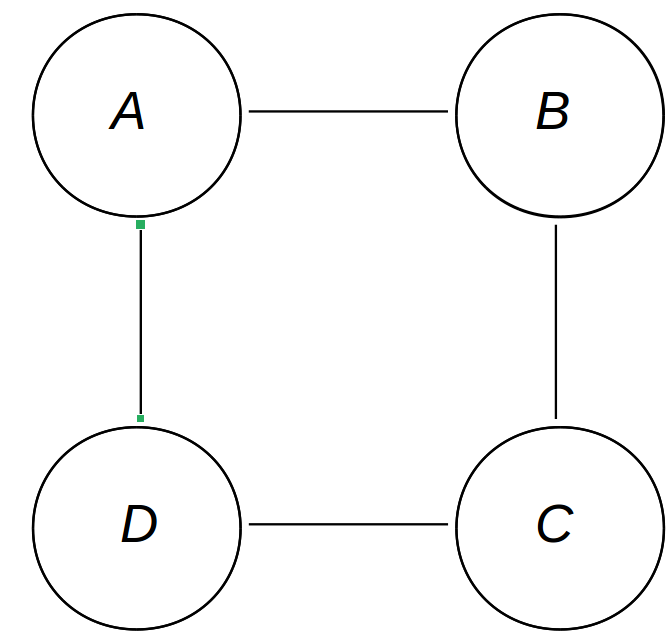
\includegraphics[width=\linewidth]{Figures/undirected_graph.png}
    \caption{Undirected graph}
  \end{subfigure}
  \begin{subfigure}[b]{0.25\linewidth}
    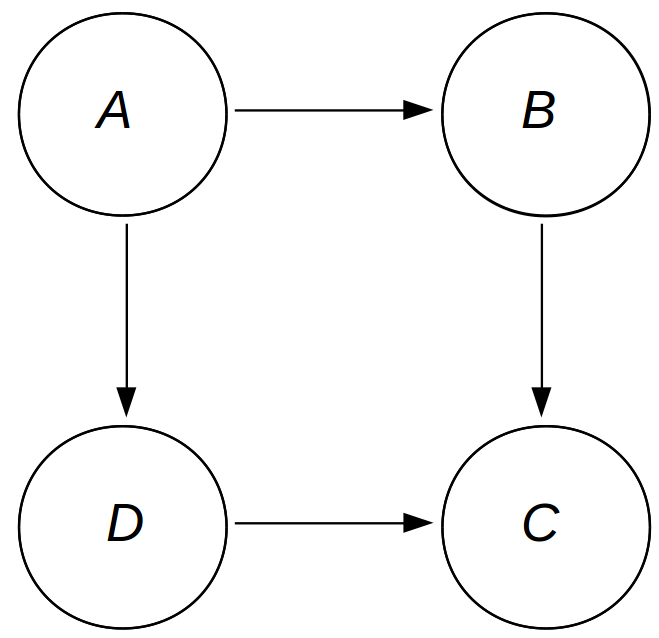
\includegraphics[width=\linewidth]{Figures/directed_graph.png}
    \caption{Directed graph}
  \end{subfigure}
  \caption{}
  \label{fig:comGraphs}
\end{figure}
\section{Bayesian PGMs}
Bayesian networks consists of random variables in the form of nodes and are connected by directed edges. Nodes that are not directly connected to each other, are considered independent. Relationships between nodes are indicated as CPDs, thus each node can be associated with a CPD
\begin{equation}
x_i \sim p(x_i|Par(x_i)),
\end{equation}
where $Par(x_i)$ indicates the parent of node $x_i$.

CPDs can be written as a factors. A factor is a function that takes a number of random variables as arguments and is defined as
\begin{equation}
\phi_i(x_i, Par(x_i)) = p(x_i|Par(x_i)),
\end{equation}
where the scope of a factor is its arguments 
\begin{equation}
Scope\{\phi_i\} = \{x_i, Par(x_i)\}.
\end{equation}
The concept of a factor is important that will be used in the rest of the report.

Figure \ref{fig:bays_pgm} is an example of a Bayesian network with seven nodes labelled from $a$ to $c$. Each node is associated with a CPD. Directed edges between nodes are indicated with arrows.
\begin{figure}[H]
  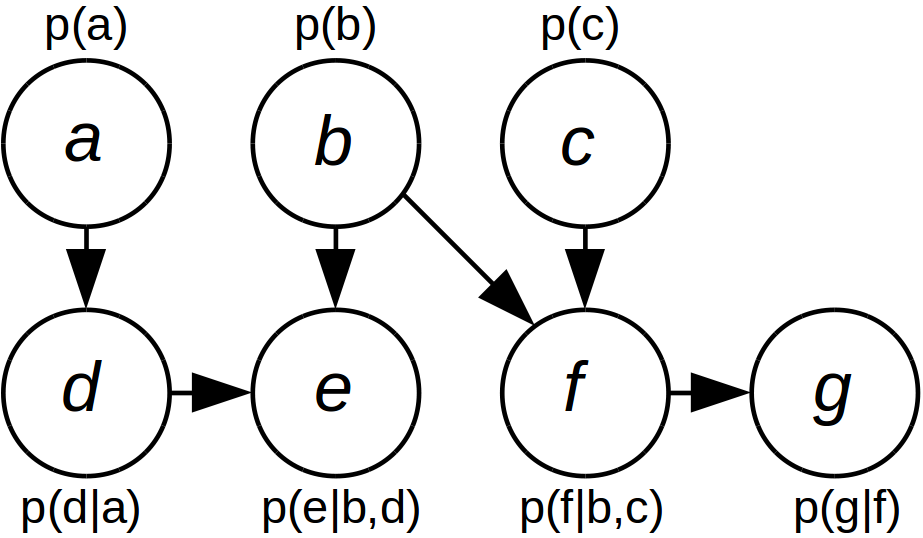
\includegraphics[width=0.5\linewidth]{Figures/bayesian_pgm.png}
  \centering
  \caption{Bayesian PGM}
  \label{fig:bays_pgm}
\end{figure}
The chain rule specifies that the joint probability density distribution of all the variables in a Bayesian network can be found by finding the product of all the CPDs associated with nodes~\citep{koller} and is defined as
\begin{equation}
p(x_1, ..., x_n) = \prod_i p(x_i|Par(x_i)).
\end{equation}
The chain rule can be applied to the Bayesian network in Figure \ref{fig:bays_pgm}
\begin{equation}
\begin{split}
p(a,b,c,d,e,f,g) & = p(a)p(b)p(c)p(d|a)p(e|b,d)p(f|b,c)p(g|f)\\
& = \phi_a(a)\phi_b(b)\phi_c(c)\phi_d(d,a)\phi_e(e,b,d)\phi_f(f,b,c)\phi_g(g,f).
\end{split}
\end{equation}
A marginal PDF of the subset of variables $a$, $b$ and $c$ can be found by integrating over the remaining variables
\begin{equation}
p(a,b,c) = \int\int\int\int p(a,b,c,d,e,f,g)dd\,de\,df\,dg.
\end{equation}
\section{Cluster Graphs}
The next step is to reason about variables of a Bayesian network. Various methods can be used to inference a Bayesian network, one method is to construct a cluster graph. The cluster graph consists of clusters connected by undirected edges.

Clusters can be formed by grouping factors together such that each cluster is subset of the variables of the Bayesian network
\begin{equation}
C_i \subseteq \{x_1, ..., x_n\}.
\end{equation}
The undirected edges between clusters are called sepsets and are responsible for passing messages between clusters. A sepset between two clusters contains information about variables that are common to both clusters and is defined as
\begin{equation}
S_{i,j} \subseteq C_i \cap C_j.
\end{equation}
There are multiple ways to construct clusters, but it should adhere to two requirements~\citep{koller}:

1. Family preservation requires that every factor $\phi_k$ in a set of factors $\Phi$ should be accommodated by a cluster, thus
\begin{equation}
Scope[{\phi}_k] \subseteq C_i.
\end{equation}

2. The running intersection property states that there exists an unique path connecting a pair of clusters containing the same variable $x$, and every cluster and sepset along the path also contain $x$. This path allows clusters to share their beliefs of $x$. In other words, for any variable $x$, the set of sepsets and clusters containing $x$ form a tree~\citep{koller}. This prevents feedback loops and thus counters the phenomena where cluster's reinforce their own beliefs of variables.

Figure \ref{fig:bays_pgm} is updated in Figure \ref{fig:cluster_bound} where CPDs is replaced with factors and possible cluster boundaries are indicated with dashed rectangles. Note that there are other ways to construct the cluster graph.
\begin{figure}[H]
  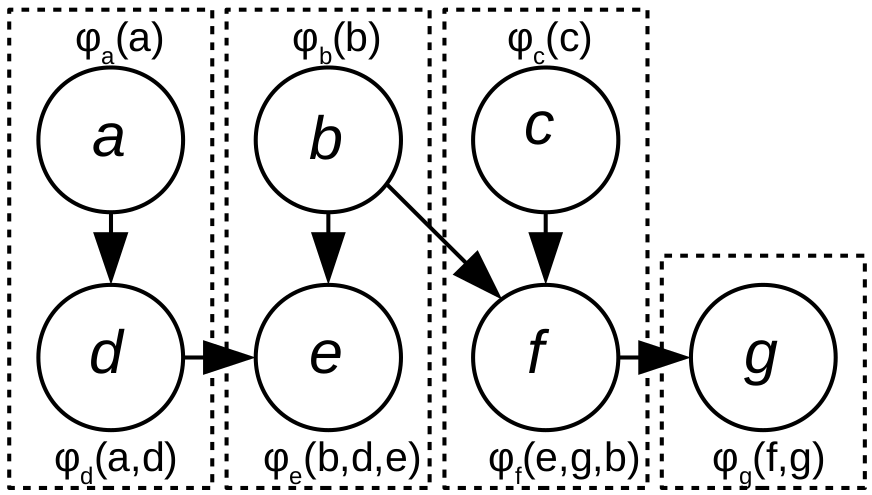
\includegraphics[width=0.6\linewidth]{Figures/cluster_divisions.png}
  \centering
  \caption{Bayesian PGM with cluster boundaries}
  \label{fig:cluster_bound}
\end{figure}

The initial belief of a cluster can be calculated by finding the product of all the factors inside the cluster.~\citep{koller}. The initial belief of a cluster is defined as
\begin{equation}
\psi_i(C_i) = \prod_{k}\phi_k.
\end{equation}
Figure \ref{fig:cluster_bound} is updated in Figure \ref{fig:clustergraph}. Clusters are indicated by ellipsis. Initial beliefs are calculated and shown inside the ellipsis. Sepsets are indicated by rectangles.
\begin{figure}[H]
  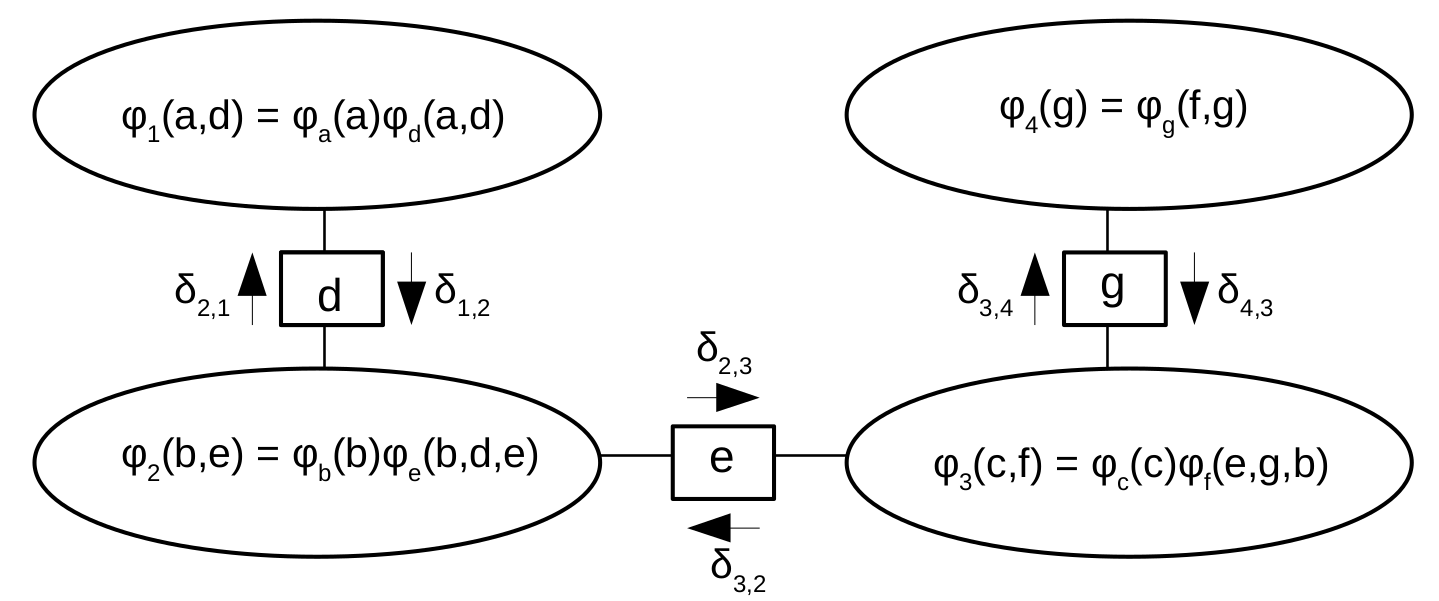
\includegraphics[width=0.7\linewidth]{Figures/clustergraph.png}
  \centering
  \caption{Cluster graph}
  \label{fig:clustergraph}
\end{figure}
\section{Message Passing}
Clusters can share beliefs of common variables with messages passing. Messages are associated with sepsets. An outgoing message of a cluster can be calculated by multiplying the cluster with all the incoming messages and then integrating over the variables that are not in the sepset.
\\Thus, messages can be calculated accordingly~\citep{koller}
\begin{equation}
\delta_{i\to j}(S_{i,j}) = \int_{C_i - S_{i,j}}\psi_i \times \prod_{k\ne j} \delta_{k\to i}(S_{k,i}).
\end{equation}
Applying to the cluster graph in Figure \ref{fig:clustergraph}:
\begin{equation}\label{eq:del12}
\delta_{1,2}(d) = \int_a \psi_1(a,d)da
\end{equation}
\begin{equation}
\delta_{2,3}(b) = \int_d \int_e \delta_{1,2}(d)\psi_2(b,d,e)dd\ de
\end{equation}
\begin{equation}
\delta_{3,4}(f) = \int_b \int_c \delta_{2,3}(b)\psi_3(b,c,f)db\ dc
\end{equation}
\begin{equation}
\delta_{4,3}(f) = \int_g \psi_4(f,g)dg
\end{equation}
\begin{equation}
\delta_{3,2}(b) = \int_c \int_f \delta_{4,3}(f)\psi_3(b,c,f)dc\ df
\end{equation}
\begin{equation}
\delta_{2,1}(d) = \int_b \int_e \delta_{3,2}(b)\psi_2(b,d,e)db\ de
\end{equation}
Sometimes the value of a RV in a PGM is known, in other words there is evidence of a RV available. Evidence of random variables is available to the entire PGM and after evidence of a RV is inferred the RV itself doesn't appear in the PGM any more. Evidence is indicated by a capital letter, thus $X$ is evidence of the RV $x$. Evidence is used to reduce a PDF before calculating messages.

In Equation \ref{eq:evidence} an out going message $\delta_{i \to j}(y)$ is calculated. Evidence of $x$ is available and is indicated as $X$. The evidence of $x$ is used to reduce the cluster $\psi_i$ before multiplying it with all incoming messages and integrating over $z$.
\begin{equation}\label{eq:evidence}
\delta_{i\to j}(y) = \int_{z}\psi_i(x = X, y, z) \times \prod_{k\ne j} \delta_{k\to i}(S_{k,i})
\end{equation}
After all the incoming messages of a cluster have been determined, the joint distribution of a cluster can be calculated by multiplying the cluster's initial belief with all of the incoming messages, and normalizing the end result. Koller and Friedman~\cite{koller} specifies this as
\begin{equation}
\beta_i(C_i) \propto \psi_i \times \prod_{k} \delta_{k \to i}(S_{k,i}).
\end{equation}

The structure of a Bayesian network consists of random variables and directed edges. Each RV is associated with a factor which describes its relationship with other random variables. One method to reason about a Bayesian network is to group factors to construct a cluster graph. Clusters of a cluster graph are connected by sepsets which allows message passing between clusters. After the initial belief of each cluster has been determined, outgoing messages of clusters can be calculated. Messages between clusters contain information about common variables and are used to update the belief clusters have of variables. The Bayesian network will be used in the next chapter to model the uncertainty of the location of a robot.
\chapter{Localisation using Probabilistic Graphical Models}
\section{Linear localisation}
\section{Non-linear localisation}
\subsection{Taylor series expansion}
\subsection{Unscented transform}
\subsection{Monte Carlo integration}

\backmatter
\bibliography{mybib}{}

\end{document}\grid
